% ============================================================
% ALCHIP INTERVIEW: AI SYSTEMS FIRST (ENGLISH FINAL VERSION)
% 16 slides, AI Systems + HBM/HBF first, followed by EDA. XeLaTeX, 16:9.
% Retain all original figures in the Overleaf project:
% SO_mapping, MO_mapping, MappingFramework, and the HBF figures.
% ============================================================
\documentclass[aspectratio=169,10pt]{beamer}
\usepackage{fontspec}
\setmainfont{Noto Sans}
\setsansfont{Noto Sans}
\usepackage{amsmath,amssymb}
\usepackage{booktabs}
\usepackage{graphicx}
\usepackage{xcolor}
\usepackage{tikz}
\usetikzlibrary{arrows.meta,positioning,calc,shapes.geometric}
\usepackage{hyperref}
\graphicspath{{./}{figures/}}

\usetheme{Madrid}
\usecolortheme{default}
\definecolor{Ink}{HTML}{243748}
\definecolor{Muted}{HTML}{667B8B}
\definecolor{Accent}{HTML}{347E74}
\definecolor{AccentBlue}{HTML}{507DAD}
\definecolor{SoftMint}{HTML}{E6F4EE}
\definecolor{SoftBlue}{HTML}{E9F2F9}
\definecolor{SoftLilac}{HTML}{F1EEF8}
\definecolor{Paper}{HTML}{FBFCFE}
\definecolor{Divider}{HTML}{D8E4EB}
\setbeamercolor{background canvas}{bg=Paper}
\setbeamercolor{normal text}{fg=Ink}
\setbeamercolor{structure}{fg=Accent}
\setbeamercolor{frametitle}{fg=Ink,bg=SoftBlue}
\setbeamercolor{block title}{fg=Ink,bg=SoftBlue}
\setbeamercolor{block body}{fg=Ink,bg=white}
\setbeamercolor{footline}{fg=Muted,bg=Paper}
\setbeamercolor{panelblue}{fg=Ink,bg=SoftBlue!68}
\setbeamercolor{panelmint}{fg=Ink,bg=SoftMint!72}
\setbeamercolor{panellilac}{fg=Ink,bg=SoftLilac!78}
\setbeamerfont{frametitle}{size=\Large,series=\bfseries}
\setbeamerfont{footline}{size=\tiny}
\setbeamertemplate{headline}{}
\setbeamertemplate{navigation symbols}{}
\setbeamertemplate{blocks}[rounded][shadow=false]
\setbeamertemplate{itemize items}[circle]
\setbeamertemplate{footline}{%
  \leavevmode\hbox{%
    \begin{beamercolorbox}[wd=\paperwidth,ht=.30cm,dp=.16cm,rightskip=.60cm plus 1fil]{footline}%
      \hfill\insertframenumber\,/\,\inserttotalframenumber
    \end{beamercolorbox}}}
\setbeamertemplate{frametitle}{%
  \nointerlineskip
  \begin{beamercolorbox}[wd=\paperwidth,ht=.77cm,dp=.18cm,leftskip=.64cm]{frametitle}%
    \usebeamerfont{frametitle}\insertframetitle
  \end{beamercolorbox}}
\newcommand{\smalllabel}[1]{{\scriptsize\bfseries\color{Accent}\MakeUppercase{#1}}}
\newcommand{\hint}[1]{{\scriptsize\color{Muted}#1}}
\newcommand{\takeaway}[1]{%
  \begin{beamercolorbox}[rounded=true,sep=0.15cm,wd=\linewidth]{block title}%
    \strut\textbf{#1}\strut
  \end{beamercolorbox}}
\newcommand{\minibadge}[2]{%
  \tikz[baseline=(badge.base)]\node[fill=#1,rounded corners=3pt,
    inner xsep=6pt,inner ysep=3pt] (badge) {\scriptsize\bfseries #2};}
\newcommand{\skillpanel}[3]{%
  \begin{beamercolorbox}[rounded=true,sep=0.11cm,wd=\linewidth]{#1}%
    \raggedright
    {\small\bfseries\color{Accent}#2\par}\vspace{0.04cm}
    {\small\color{Ink}#3\par}%
  \end{beamercolorbox}}

% Image placeholders: literal filenames are safe even with underscores.
% Keep this definition before \begin{document}.
\providecommand{\aiplaceholder}[3]{}
\renewcommand{\aiplaceholder}[3]{%
  \par\noindent
  \begin{tikzpicture}
    \node[draw=AccentBlue!55,dashed,line width=0.6pt,
      rounded corners=4pt,fill=SoftBlue!35,
      text width=\dimexpr\linewidth-0.82cm\relax,
      minimum height=#1,inner xsep=0.40cm,inner ysep=0.12cm,
      outer sep=0pt,align=center] {%
      {\small\bfseries\color{AccentBlue}IMAGE PLACEHOLDER}\par
      \vspace{0.12cm}
      {\small\color{Ink}#2\par}
      \vspace{0.10cm}
      {\scriptsize\ttfamily\color{Muted}\detokenize{#3}\par}%
    };
  \end{tikzpicture}\par
}


% Existing mapping figures are expected to be in the original Overleaf project.
% In a new project without these files, an explicit placeholder is shown
% instead of failing compilation. Copy actual figures into figures/.
\newcommand{\safeimage}[3][]{%
  \IfFileExists{#2}{\includegraphics[#1]{#2}}{%
    \IfFileExists{figures/#2}{\includegraphics[#1]{figures/#2}}{%
      \begin{tikzpicture}
        \node[draw=AccentBlue!60,fill=SoftBlue!40,dashed,
              rounded corners=3pt,text width=\dimexpr\linewidth-0.6cm\relax,
              minimum height=#3,align=center,inner sep=0.17cm] {%
          {\small\bfseries\color{AccentBlue}Existing Overleaf figure required}\\[2mm]
          {\scriptsize\ttfamily\detokenize{#2}}};
      \end{tikzpicture}%
    }%
  }%
}

\title[AI Systems / EDA]{AI Hardware Architecture \& Simulation / EDA Tool Development \& Verification}
\subtitle{MoE Inference / HBM--HBF / Hardware Simulation / Technology Mapping}
\author{Yu-Jui Liang}
\institute{National Taiwan University}
\date{}
\begin{document}
% ===========================================================
% MAIN PRESENTATION -- revised for Alchip Assembly Packaging
% AI Systems + HBM/HBF section precedes all EDA slides; discuss detailed figures as time permits.
% ===========================================================

{\setbeamertemplate{footline}{}
\begin{frame}[plain]
  \vspace*{0.76cm}
  \smalllabel{TECHNICAL INTERVIEW PORTFOLIO}\par
  \vspace{0.47cm}
{\raggedright\fontsize{21}{27}\selectfont\bfseries\color{Ink}
  AI Hardware Architecture \& Simulation\\[2mm]
  EDA Tool Development \& Verification\par}
  \vspace{0.27cm}
  {\normalsize\color{Muted}AI Memory Systems \quad / \quad Software Simulation \quad / \quad EDA Tool Development\par}
  \vspace{0.61cm}
  {\Large\mdseries\color{Ink}Yu-Jui Liang\par}
  \vspace{0.09cm}
  {\normalsize\color{Muted}M.S. in Data Science\par}
  {\small\color{Muted}National Taiwan University \quad | \quad Expected Graduation: June 2027\par}
  \vspace{0.17cm}
  {\small\color{Muted}\href{mailto:liangyujui@gmail.com}{liangyujui@gmail.com}\par}
  \vspace{0.03cm}
  {\small\color{Muted}\href{https://www.linkedin.com/in/yu-jui-liang-735a57316}{https://www.linkedin.com/in/yu-jui-liang-735a57316}\par}
  \vfill
  {\color{Accent}\rule{\textwidth}{0.7pt}}\par\vspace{0.07cm}
  {\small\bfseries\color{Muted}
    AI Hardware Architecture \quad / \quad GPU--HBM/HBF Co-design\par}
\end{frame}}

\begin{frame}{Education and Technical Background}
  \vspace{0.00cm}
  \smalllabel{01 / Background}\par\vspace{0.12cm}
  \vspace{0.16cm}
  \begin{columns}[T,onlytextwidth]
    \begin{column}{0.49\textwidth}
      \begin{beamercolorbox}[rounded=true,sep=0.21cm,wd=\linewidth]{panelblue}
        {\normalsize\bfseries\color{AccentBlue}Education}\par\vspace{0.15cm}
        {\small\bfseries National Taiwan University}\par
        {\small M.S. in Data Science}\par
        {\scriptsize\color{Muted}Sep. 2025 -- Expected Jun. 2027}\par
        \vspace{0.22cm}
        {\small\bfseries National Chengchi University}\par
        {\small B.S. in Computer Science}\par
        {\small Double Major in Electrophysics}\par
        {\scriptsize\color{Muted}2021.09 -- 2025.06}
      \end{beamercolorbox}
    \end{column}
    \begin{column}{0.49\textwidth}
      \begin{beamercolorbox}[rounded=true,sep=0.21cm,wd=\linewidth]{panelmint}
        {\normalsize\bfseries\color{Accent}Research and Engineering}\par\vspace{0.15cm}
        {\small\bfseries AI Hardware Systems}\par
        {\small GPU / HBM / HBF Memory Hierarchy}\par
        {\small Workload-Aware Performance Modeling}\par
        {\small HW/SW Co-design Exploration}\par
        \vspace{0.20cm}
        {\small\bfseries EDA Software Development}\par
        {\small Logic Synthesis / Technology Mapping}\par
        {\small C++ Tool Integration / Verification}
      \end{beamercolorbox}
    \end{column}
  \end{columns}
  \vspace{0.14cm}
\end{frame}

\begin{frame}{Professional Experience}
  \vspace{-0.06cm}
  \smalllabel{02 / Industry Experience}\par\vspace{0.10cm}
  \vspace{0.06cm}
  \begin{beamercolorbox}[rounded=true,sep=0.17cm,wd=\linewidth]{panelmint}
    {\normalsize\bfseries\color{Ink}NeoPower}\hfill
    {\scriptsize\color{Muted}Jun. 2023 -- Mar. 2025}\par
    \vspace{0.07cm}{\small\bfseries\color{Accent}Contract Software Engineer}\par\vspace{0.13cm}
    {\small\color{Ink}\textbf{Custom Simulator:} Built a simulator to reproduce operational workflows and error scenarios.}\par\vspace{0.07cm}
    {\small\color{Ink}\textbf{Software Validation:} Performed end-to-end testing, regression testing, and debugging.}\par\vspace{0.07cm}
    {\small\color{Ink}\textbf{Customer-Side Validation:} A/B testing, post-deployment checks, and log/data analysis.}\par
  \end{beamercolorbox}
  \vspace{0.10cm}
  \begin{beamercolorbox}[rounded=true,sep=0.17cm,wd=\linewidth]{panelblue}
    {\normalsize\bfseries\color{Ink}Smart Mobility Subsidiary (Inventec Group)}\hfill
    {\scriptsize\color{Muted}Apr. 2025 -- Jul. 2025}\par
    \vspace{0.07cm}{\small\bfseries\color{AccentBlue}Contract Software Engineer}\par
    \vspace{0.07cm}{\small\color{Ink}Contributed to software development, system integration, testing, and debugging.}
  \end{beamercolorbox}
\end{frame}

\begin{frame}{Projects and Research Focus}
  \vspace{0.03cm}
  \smalllabel{03 / Portfolio Roadmap}\par\vspace{0.10cm}
  \takeaway{AI hardware architecture first, followed by EDA software development and validation.}
  \vspace{0.16cm}
  \begin{beamercolorbox}[rounded=true,sep=0.15cm,wd=\linewidth]{panelmint}
    {\small\bfseries\color{Accent}01 \quad AI Hardware Systems}\par\vspace{0.02cm}
    {\normalsize\bfseries Workload-Aware HBM/HBF Memory Architecture Exploration}\par
    {\small MoE Inference / Hardware Modeling / Performance--Power--Endurance Trade-offs}
  \end{beamercolorbox}
  \vspace{0.14cm}
  \begin{beamercolorbox}[rounded=true,sep=0.15cm,wd=\linewidth]{panelblue}
    {\small\bfseries\color{AccentBlue}02 \quad EDA Tool Development}\par\vspace{0.02cm}
    {\normalsize\bfseries Multi-Output Standard-Cell Technology Mapping}\par
    {\small C++ / Boolean Matching / Optimization / Correctness Validation}
  \end{beamercolorbox}
  \vspace{0.14cm}
  {\small\color{Muted}Shared skills: Simulation, Software Development, Quantitative Evaluation, and Testing.}
\end{frame}


% ===========================================================
% PROJECT 01 COVER -- slide 5 (before MoE memory bottleneck)
% ===========================================================
\begin{frame}{AI Hardware Systems: Project Overview}
  \vspace{0.01cm}
  \smalllabel{04 / AI Systems -- Project Introduction}\par\vspace{0.10cm}
  {\LARGE\bfseries\color{Ink}Workload-Aware GPU Memory Architecture}\par
  \vspace{0.05cm}
  {\normalsize\color{Muted}Hardware/Software Co-design \quad / \quad System-Level Simulation}\par
  \vspace{0.05cm}
  \takeaway{Co-design GPU memory architectures for the compute and memory needs of targeted AI models.}
  \vspace{0.07cm}
  \begin{center}
  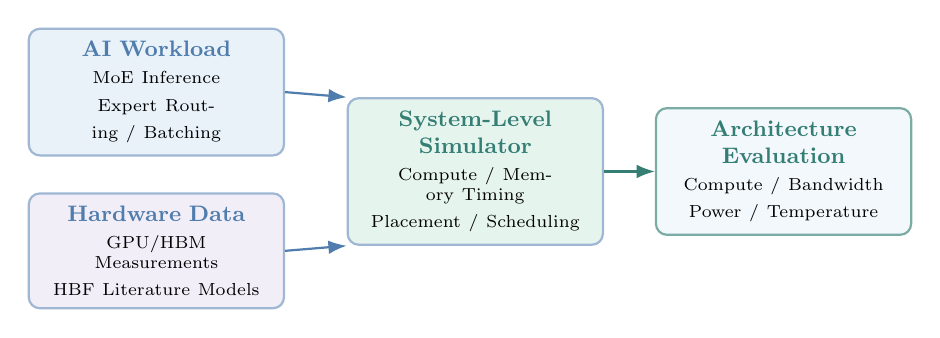
\begin{tikzpicture}[>=Latex,font=\small,line width=.8pt,scale=.90,transform shape]
    \tikzset{
      coverbox/.style={draw=AccentBlue!55,rounded corners=4pt,
        minimum height=1.06cm,text width=3.25cm,align=center,inner sep=5pt},
      resultbox/.style={draw=Accent!65,rounded corners=4pt,
        minimum height=1.18cm,text width=3.25cm,align=center,inner sep=5pt}
    }
    \node[coverbox,fill=SoftBlue] (workload) at (-4.45,1.12)
      {{\bfseries\color{AccentBlue}AI Workload}\par\vspace{1mm}
       {\scriptsize MoE Inference\\Expert Routing / Batching}};
    \node[coverbox,fill=SoftLilac] (hardware) at (-4.45,-1.12)
      {{\bfseries\color{AccentBlue}Hardware Data}\par\vspace{1mm}
       {\scriptsize GPU/HBM Measurements\\HBF Literature Models}};
    \node[coverbox,fill=SoftMint,minimum height=1.32cm] (sim) at (0.05,0)
      {{\bfseries\color{Accent}System-Level Simulator}\par\vspace{1mm}
       {\scriptsize Compute / Memory Timing\\Placement / Scheduling}};
    \node[resultbox,fill=SoftBlue!55] (output) at (4.40,0)
      {{\bfseries\color{Accent}Architecture Evaluation}\par\vspace{1mm}
       {\scriptsize Compute / Bandwidth\\Power / Temperature}};
    \draw[->,AccentBlue,thick] (workload.east) -- (sim.north west);
    \draw[->,AccentBlue,thick] (hardware.east) -- (sim.south west);
    \draw[->,Accent,thick] (sim.east) -- (output.west);
  \end{tikzpicture}
  \end{center}
  \vspace{0.00cm}
  {\scriptsize\color{Muted}Simulation uses available hardware specifications and measurements; HBF uses published models and design parameters.}
\end{frame}

\begin{frame}{MoE Inference: Memory Bottleneck}
  \vspace{0.00cm}
  \smalllabel{05 / AI Systems -- Motivation}\par\vspace{0.07cm}
  \takeaway{MoE reduces computation per token, but large expert weights must still be stored and transferred as needed.}
  \vspace{0.04cm}
  \begin{columns}[c,onlytextwidth]
    \begin{column}{0.56\textwidth}
      \begin{center}
      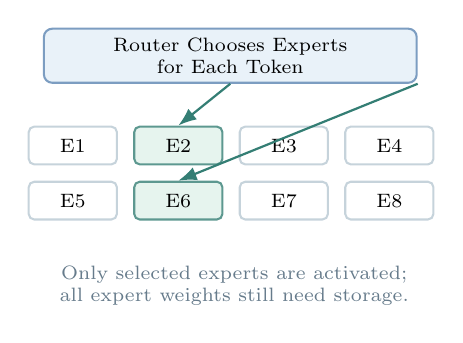
\begin{tikzpicture}[>=Latex, font=\scriptsize, line width=.75pt]
        \node[draw=AccentBlue!75,fill=SoftBlue,rounded corners=3pt,
          text width=4.5cm,minimum height=.59cm,align=center] (router) at (0,2.12)
          {Router Chooses Experts\\for Each Token};
        \foreach \i in {1,...,8}{
          \pgfmathtruncatemacro{\xindex}{mod(\i-1,4)}
          \pgfmathtruncatemacro{\yindex}{int((\i-1)/4)}
          \pgfmathsetmacro{\xpos}{-2.0+1.34*\xindex}
          \pgfmathsetmacro{\ypos}{0.98-0.70*\yindex}
          \ifnum\i=2
            \node[draw=Accent!80,fill=SoftMint,rounded corners=2pt,minimum width=1.12cm,
              minimum height=.48cm] (e\i) at (\xpos,\ypos) {E\i};
          \else\ifnum\i=6
            \node[draw=Accent!80,fill=SoftMint,rounded corners=2pt,minimum width=1.12cm,
              minimum height=.48cm] (e\i) at (\xpos,\ypos) {E\i};
          \else
            \node[draw=Divider!90!Ink,fill=white,rounded corners=2pt,minimum width=1.12cm,
              minimum height=.48cm] (e\i) at (\xpos,\ypos) {E\i};
          \fi\fi
        }
        \draw[->,Accent,thick] (router.south) -- (e2.north);
        \draw[->,Accent,thick] (router.south east) -- (e6.north);
        \node[align=center,text=Muted,font=\scriptsize] at (.05,-.80)
          {Only selected experts are activated;\\all expert weights still need storage.};
      \end{tikzpicture}
      \end{center}
    \end{column}
    \begin{column}{0.41\textwidth}
      \skillpanel{panelblue}{Compute Efficiency}{Each token activates only a subset of experts, reducing computation.}
      \vspace{0.10cm}
      \skillpanel{panellilac}{Memory Capacity}{The full set of expert weights may exceed HBM capacity.}
      \vspace{0.10cm}
      \skillpanel{panelmint}{Transfer Bottleneck}{Loading experts from host DRAM / SSD may stall GPU execution.}
    \end{column}
  \end{columns}
  \vspace{0.01cm}
  % Discussion: residency depends on model size, batching, and runtime policy.
\end{frame}

\begin{frame}{Hybrid HBM/HBF: Candidate Memory Architecture}
  \vspace{0.02cm}
  \smalllabel{06 / AI Systems -- Architecture}\par\vspace{0.09cm}
  \takeaway{Trade some HBM stack sites for higher HBF capacity and explore package-local memory trade-offs.}
  \vspace{0.08cm}
  \begin{columns}[c,onlytextwidth]
    \begin{column}{0.67\textwidth}
      \begin{center}
        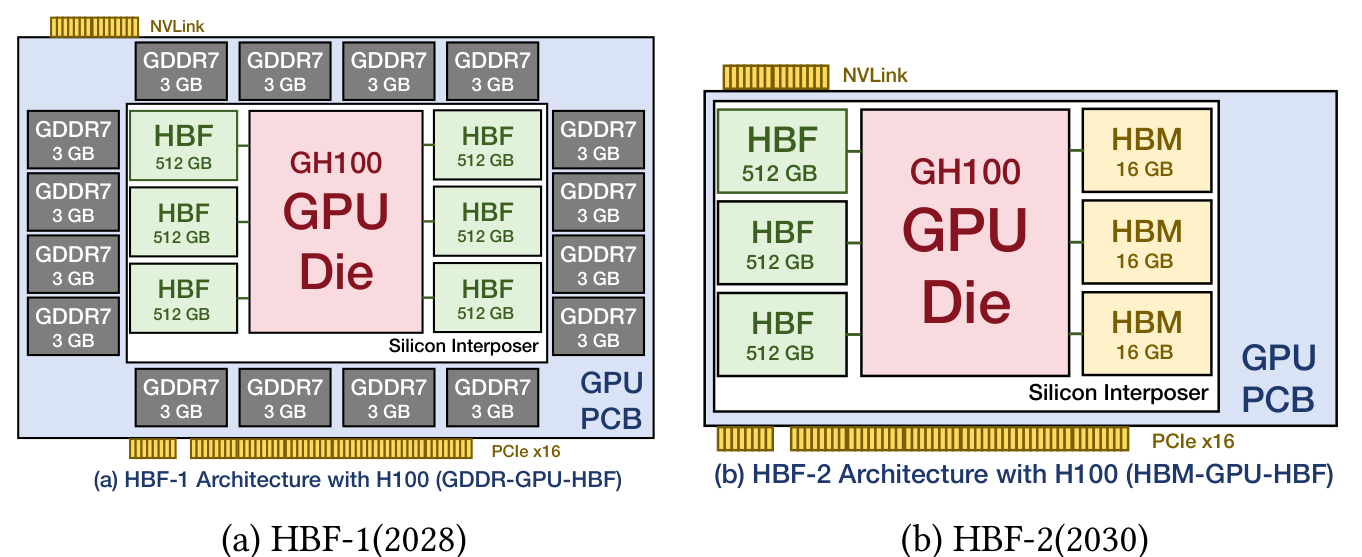
\includegraphics[width=\linewidth,height=3.90cm,keepaspectratio]{Figure_01_HBF1_HBF2_slide.png}
      \end{center}
    \end{column}
    \begin{column}{0.30\textwidth}
      \skillpanel{panelblue}{Modeled HBF-2 Setup}{3 HBM + 3 HBF; 48 GB HBM + 1.5 TB HBF.}
      \vspace{0.05cm}
      \skillpanel{panelmint}{Capacity Benefit}{Larger on-package memory capacity.}
      \vspace{0.05cm}
      \skillpanel{panellilac}{Architecture Trade-off}{Reduced HBM capacity and bandwidth.}
    \end{column}
  \end{columns}
  \vspace{0.00cm}
  % Reference only (not displayed in slides): Li et al., arXiv:2608.11668, Fig. 1; modeled from KAIST TERA Lab's HBF roadmap (not a commercial HBF-2 product).
\end{frame}

\begin{frame}{HBF Physical Organization: 2.5D/3D Packaging}
  \vspace{0.08cm}
  \smalllabel{07 / AI Systems -- Packaging}\par\vspace{0.09cm}
  \takeaway{HBF integrates stacked NAND, TSVs, a base die, and an interposer in an advanced package.}
  \begin{center}
    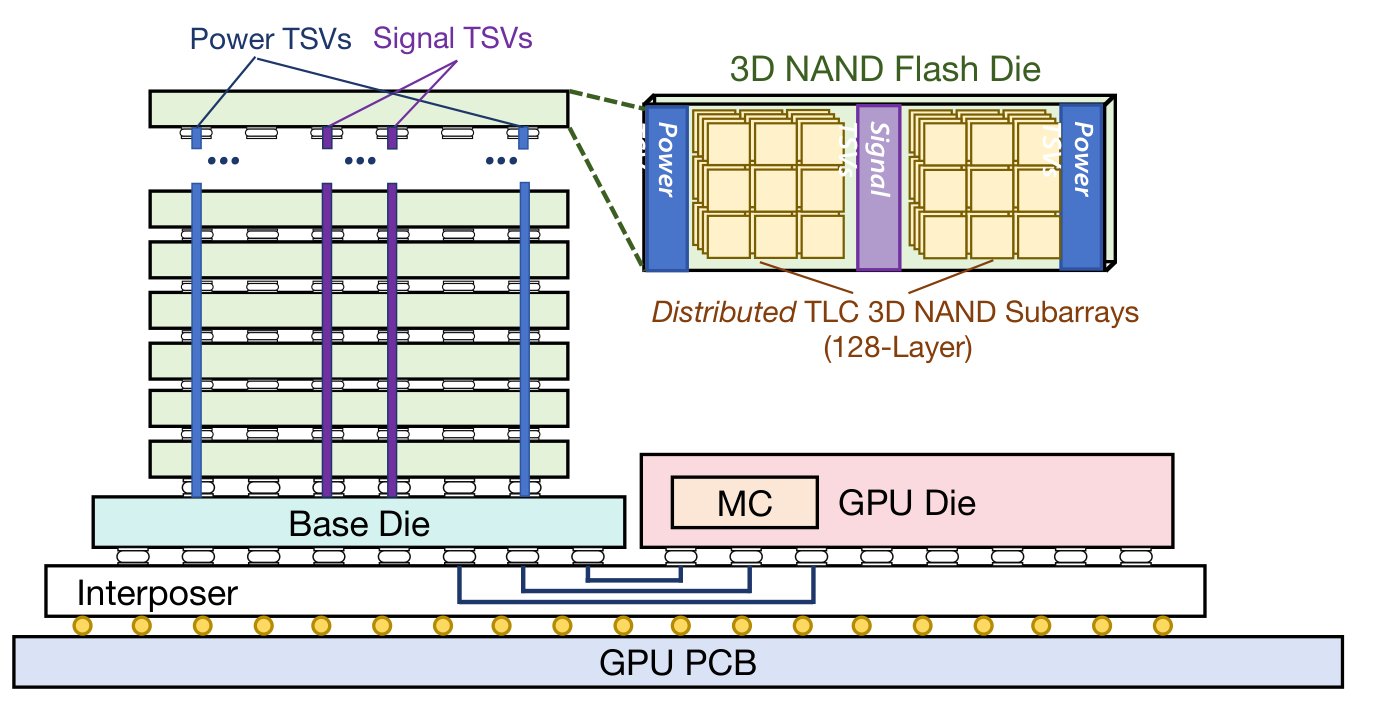
\includegraphics[width=0.86\linewidth,height=4.30cm,keepaspectratio]{Figure_02_HBF_package_slide.png}
  \end{center}
  % Reference only (not displayed in slides): Li et al., arXiv:2608.11668, Fig. 2. Reference diagram; not original layout or package design work.
\end{frame}

\begin{frame}{Software Simulation: Architecture Exploration}
  \vspace{0.01cm}
  \smalllabel{08 / AI Systems -- Methodology}\par\vspace{0.11cm}
  \takeaway{Use software simulation to compare memory configurations and MoE workloads before hardware implementation.}
  \vspace{0.09cm}
  \begin{columns}[T,onlytextwidth]
    \begin{column}{0.31\textwidth}
      \skillpanel{panelblue}{Workload Inputs}{MoE model, expert selection, request arrivals, context length, and batch size.}
      \vspace{0.18cm}
      \skillpanel{panelblue}{Hardware Parameters}{GPU compute, stack count, capacity, latency, bandwidth, and power.}
    \end{column}
    \begin{column}{0.06\textwidth}
      \vspace{1.55cm}
      \begin{center}{\Large\color{AccentBlue}$\rightarrow$}\end{center}
    \end{column}
    \begin{column}{0.30\textwidth}
      \begin{beamercolorbox}[rounded=true,sep=0.18cm,wd=\linewidth]{panelmint}
        {\large\bfseries\color{Accent}System-Level Simulator}\par\vspace{0.15cm}
        {\small Compute / Transfer Timing}\par\vspace{0.10cm}
        {\small Data Placement / Migration}\par\vspace{0.10cm}
        {\small Scheduling / Prefetch}\par\vspace{0.10cm}
        {\small Thermal / Endurance Models}
      \end{beamercolorbox}
    \end{column}
    \begin{column}{0.06\textwidth}
      \vspace{1.55cm}
      \begin{center}{\Large\color{AccentBlue}$\rightarrow$}\end{center}
    \end{column}
    \begin{column}{0.25\textwidth}
      \skillpanel{panellilac}{Evaluation Metrics}{Throughput, TTFT/TPOT, SLO goodput, bandwidth, temperature, and lifetime.}
      \vspace{0.15cm}
      \skillpanel{panelmint}{Software Policies}{Weight placement, batching, and HBM watermark parameter sweeps.}
    \end{column}
  \end{columns}

\end{frame}

\begin{frame}{HW/SW Co-design: Data Placement and Constraints}
  \vspace{0.03cm}
  \smalllabel{09 / AI Systems -- Design Hypotheses}\par\vspace{0.10cm}
  \takeaway{Capacity alone is not enough: data reuse, transfer stalls, power, and write endurance also matter.}
  \vspace{0.00cm}
  \begin{columns}[c,onlytextwidth]
    \begin{column}{0.55\textwidth}
      \begin{center}
        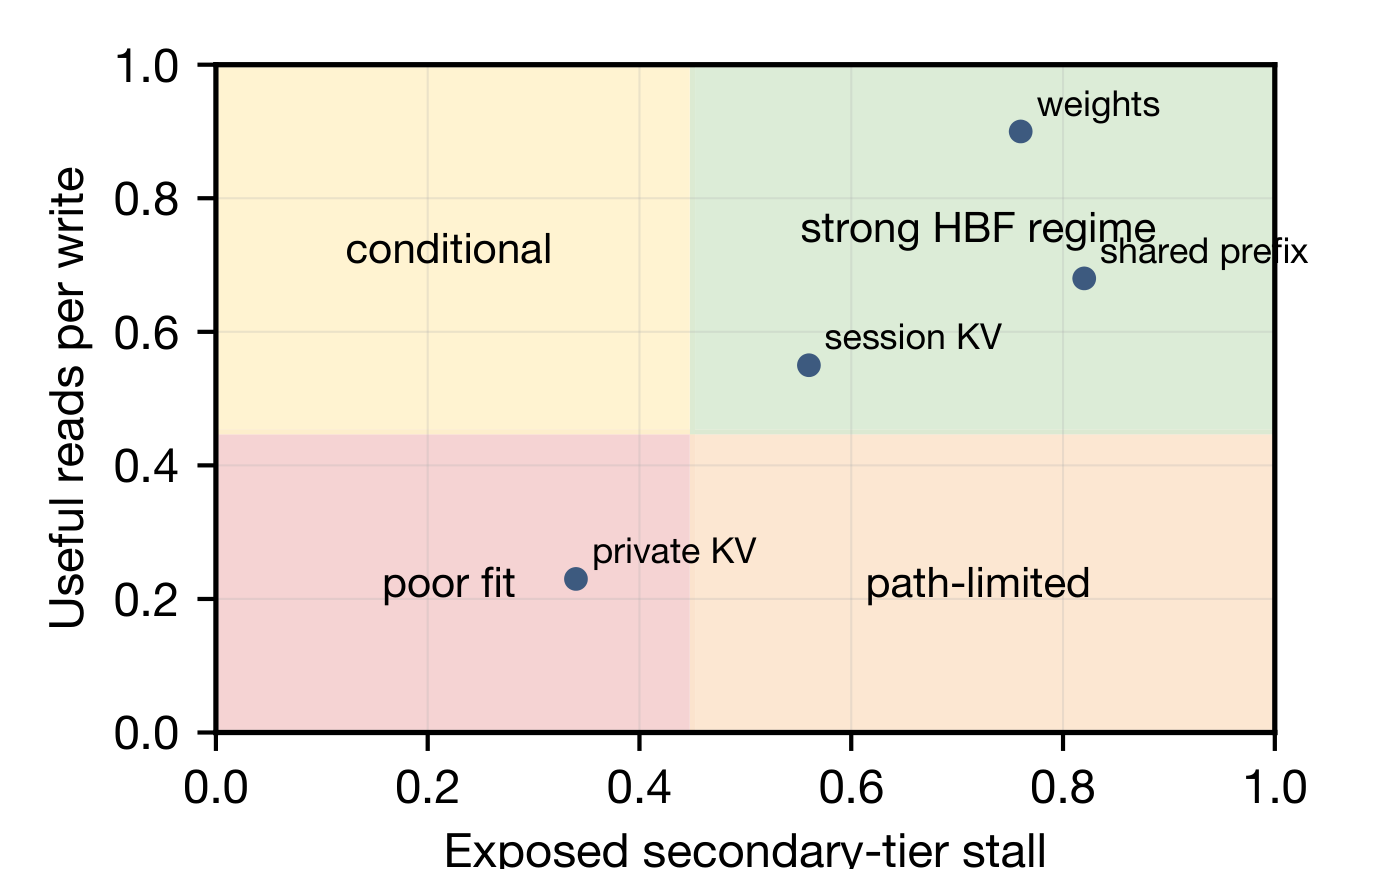
\includegraphics[height=4.65cm,width=\linewidth,keepaspectratio]{Figure_12_HBF_placement_slide.png}
      \end{center}
    \end{column}
    \begin{column}{0.42\textwidth}
      \skillpanel{panelmint}{HBM: Latency-Sensitive Data}{Keep active experts and frequently updated KV cache in HBM.}
      \vspace{0.06cm}
      \skillpanel{panelblue}{HBF: Read-Mostly Data}{Evaluate expert weights and reusable shared prefixes for HBF.}
      \vspace{0.06cm}
      \skillpanel{panellilac}{Policies and Reliability}{Explore prefetching, scheduling, HBM watermarks, thermal caps, and P/E wear.}
    \end{column}
  \end{columns}
  \vspace{0.06cm}
  % Reference only (not displayed): Li et al., arXiv:2608.11668, Fig. 12. This is not a result from our study.
\end{frame}

\begin{frame}{Thermal-constrained HBF Bandwidth}
  \vspace{-0.02cm}
  \smalllabel{10 / AI Systems -- Thermal Limits}\par\vspace{0.07cm}
  \takeaway{Sustained bandwidth is limited by thermal constraints, not just peak interface bandwidth.}
  \vspace{0.02cm}
  \begin{center}
    % Keep the full image (including bottom x-axis); no trim or clipping.
    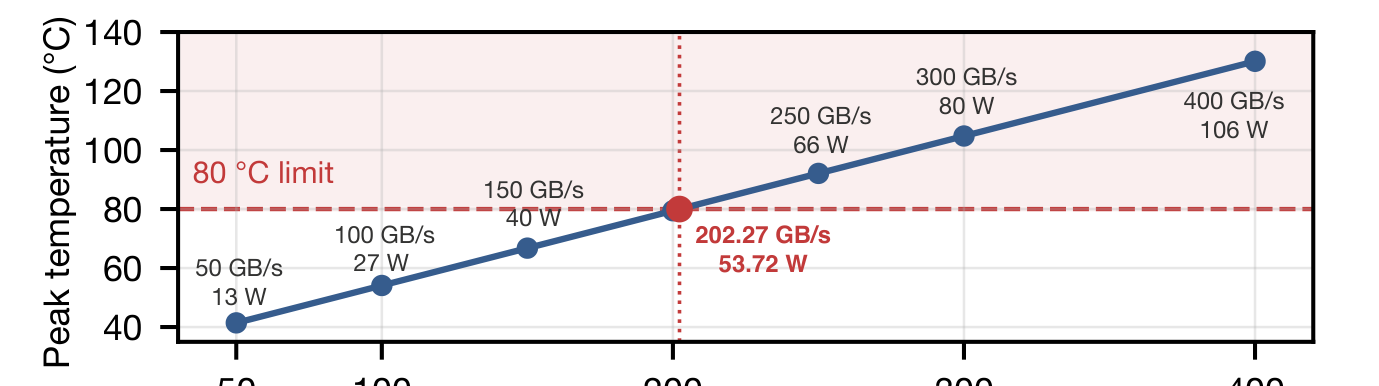
\includegraphics[width=0.85\linewidth,height=3.45cm,keepaspectratio]{Figure_10_thermal_curve_slide.png}
  \end{center}
  % Extra clearance below the plot prevents x-axis labels touching the next panel.
  \vspace{0.22cm}
  \skillpanel{panelmint}{Literature Model}{In the paper model, a 16-Hi TLC HBF stack sustains about 202 GB/s near 80\,$^{\circ}$C.}
  \vspace{0.02cm}
  % Reference only (not displayed in slides): Li et al., arXiv:2608.11668, Fig. 10(a). Assumption-dependent prediction, not measured HBF hardware.
\end{frame}

\begin{frame}{Technology Mapping: Why Multi-Output Cells?}
  \vspace{0.05cm}
  \smalllabel{11 / EDA Project -- Motivation}
  \vspace{0.12cm}
  \takeaway{Logic synthesis maps functions to standard cells; multi-output cells may share logic.}
  \vspace{-0.25cm}
  \begin{columns}[T,onlytextwidth]
    \begin{column}{0.492\textwidth}
      \minibadge{SoftLilac}{Single-Output Mapping}
      \vspace{0.02cm}
      \begin{center}
        \safeimage[width=\linewidth,height=3.95cm,keepaspectratio,trim=0 105bp 0 250bp,clip]{SO_mapping.png}{3.75cm}
      \end{center}
      \vspace{-0.18cm}
      % The SO circuit diagram already illustrates the separate-cell implementation.
    \end{column}
    \begin{column}{0.492\textwidth}
      \minibadge{SoftMint}{Multi-Output Mapping}
      \vspace{0.02cm}
      \begin{center}
        \safeimage[width=\linewidth,height=3.95cm,keepaspectratio,trim=0 180bp 0 175bp,clip]{MO_mapping.png}{3.75cm}
      \end{center}
      \vspace{-0.18cm}
      % The MO circuit diagram already illustrates the joint-cell implementation.
    \end{column}
  \end{columns}
  \vspace{-0.16cm}
  \begin{center}
    {\small\bfseries\color{Accent}Potential benefit: }
    {\small\color{Ink}Shared logic may reduce both area and delay.}
  \end{center}
\end{frame}

\begin{frame}{ABC Mapper: Multi-Output Mapping Extension}
  \vspace{0.06cm}
  \smalllabel{12 / EDA Project -- Implementation}\par
  \vspace{0.10cm}
  \takeaway{Added multi-output candidate discovery and output-pair binding to ABC.}
  \vspace{-0.08cm}
  \begin{center}
    \safeimage[width=\linewidth,height=4.70cm,keepaspectratio,
        trim=0 80bp 0 132bp,clip]{MappingFramework.png}{4.2cm}%
  \end{center}
\end{frame}

\begin{frame}{Experimental Results: Area-Delay Product}
  \vspace{-0.07cm}
  \smalllabel{13 / EDA Project -- Evaluation}
  \vspace{0.10cm}
  {\small\color{Muted}30 benchmark cases \quad | \quad 7nm ASAP7 \quad | \quad GMean normalized ADP}
  \vspace{0.02cm}
  \begin{columns}[T,onlytextwidth]
    \begin{column}{0.58\textwidth}
      {\normalsize\bfseries Normalized ADP (Area--Delay Product)}\par
      \vspace{0.08cm}
      \centering

      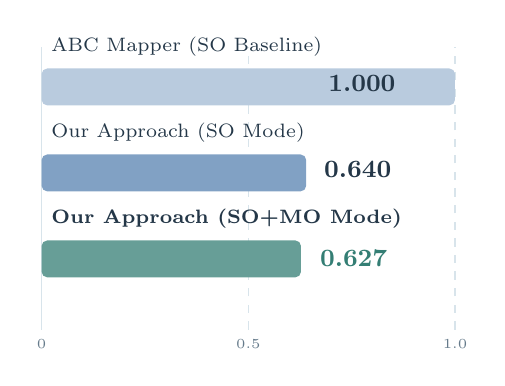
\begin{tikzpicture}[x=5.25cm,y=.78cm]
        % guide lines for 0%, 50%, 100%
        \draw[Divider,thin] (0,0) -- (0,4.6);
        \draw[Divider,dashed,thin] (.5,0) -- (.5,4.6);
        \draw[Divider,dashed,thin] (1,0) -- (1,4.6);
        \foreach \x/\t in {0/0,0.5/0.5,1/1.0}{\node[font=\tiny,text=Muted,anchor=north] at (\x,0) {\t};}
        % value bars, true to scale
        \fill[AccentBlue!40,rounded corners=2pt] (0,3.65) rectangle (1,4.25);
        \fill[AccentBlue!72,rounded corners=2pt] (0,2.25) rectangle (.6400,2.85);
        \fill[Accent!75,rounded corners=2pt] (0,.85) rectangle (.6274,1.45);
        % visible values on bars
        \node[font=\small\bfseries,text=Ink,anchor=west] at (.67,4.0) {1.000};
        \node[font=\small\bfseries,text=Ink,anchor=west] at (.66,2.60) {0.640};
        \node[font=\small\bfseries,text=Accent,anchor=west] at (.65,1.15) {0.627};
        % row captions
        \node[font=\scriptsize,text=Ink,anchor=south west] at (0,4.29) {ABC Mapper (SO Baseline)};
        \node[font=\scriptsize,text=Ink,anchor=south west] at (0,2.89) {Our Approach (SO Mode)};
        \node[font=\scriptsize\bfseries,text=Ink,anchor=south west] at (0,1.49) {Our Approach (SO+MO Mode)};
      \end{tikzpicture}
    \end{column}
    \begin{column}{0.37\textwidth}
      \vspace{0.10cm}
      \begin{beamercolorbox}[rounded=true,sep=0.19cm,wd=\linewidth]{block title}
        {\fontsize{21}{23}\selectfont\bfseries\color{Accent}37.3\%}\\[1.5mm]
        {\small ADP reduction vs. ABC baseline}
      \end{beamercolorbox}
      \vspace{0.22cm}
      \begin{beamercolorbox}[rounded=true,sep=0.19cm,wd=\linewidth]{block title}
        {\fontsize{21}{23}\selectfont\bfseries\color{AccentBlue}2.0\%}\\[1.5mm]
        {\small Further improvement vs. SO mode}
      \end{beamercolorbox}

    \end{column}
  \end{columns}
  \vspace{0.05cm}
  {\scriptsize\color{Muted}The 30-case results are from an earlier bridge-based flow; ABC-native MO discovery was developed later.}\par
\end{frame}

\begin{frame}{Software Engineering: Verification and Evaluation}
  \vspace{0.03cm}
  \smalllabel{14 / Engineering Practices}\par\vspace{0.10cm}
  \takeaway{Preserve logic correctness and benchmark reproducibility when optimizing tools.}
  \vspace{0.16cm}
  \begin{columns}[T,onlytextwidth]
    \begin{column}{0.485\textwidth}
      \begin{beamercolorbox}[rounded=true,sep=0.19cm,wd=\linewidth]{panelblue}
        {\large\bfseries\color{AccentBlue}Correctness}\par\vspace{0.14cm}
        {\small\bfseries Regression Testing}\par
        {\small Start with small smoke tests after each change.}\par
        \vspace{0.12cm}
        {\small\bfseries Boolean Equivalence}\par
        {\small Use combinational equivalence checking (CEC) to compare the original circuit and mapped netlist.}\par
        \vspace{0.12cm}
        {\small\bfseries Backward Compatibility}\par
        {\small Preserve the existing single-output mapping flow.}
      \end{beamercolorbox}
    \end{column}
    \begin{column}{0.485\textwidth}
      \begin{beamercolorbox}[rounded=true,sep=0.19cm,wd=\linewidth]{panelmint}
        {\large\bfseries\color{Accent}Reproducibility}\par\vspace{0.14cm}
        {\small\bfseries Quantitative Comparison}\par
        {\small Use fixed benchmarks and baselines for controlled comparisons.}\par
        \vspace{0.12cm}
        {\small\bfseries Hardware-Aware Metrics}\par
        {\small Use cell-library area/delay and normalized ADP.}\par
        \vspace{0.12cm}
        {\small\bfseries Resource Discipline}\par
        {\small Bound the search space; monitor runtime and peak memory.}
      \end{beamercolorbox}
    \end{column}
  \end{columns}
\end{frame}

{\setbeamertemplate{footline}{}
\begin{frame}[plain]
  \vfill
  \begin{center}
    {\fontsize{34}{43}\selectfont\bfseries\color{Ink}Thank You}\par
    \vspace{0.28cm}
    {\Large\color{Accent}Q\&A}\par
  \end{center}
  \vfill
\end{frame}}



\end{document}